\exer{Traversée d'une rivière avec un loup, une chèvre et un choux}
\begin{flushright}
\textit{Ressources de KOVALTCHOUK Thibaut.}
\end{flushright}
\setcounter{numques}{0}
Sur la rive d'un fleuve se trouvent un loup, une chèvre, un chou et un passeur. Le problème consiste à tous les faire passer sur l'autre rive à l'aide d'une barque, menée par le passeur, en respectant les règles suivantes~:
\begin{itemize}
	\item la chèvre et le chou ne peuvent pas rester sur la même rive sans le passeur~;
	\item la chèvre et le loup ne peuvent pas rester sur la même rive sans le passeur~;
	\item le passeur ne peut mettre qu'un seul \og~passager~\fg{} avec lui.
\end{itemize}

\begin{figure}[h]
	\begin{center}
		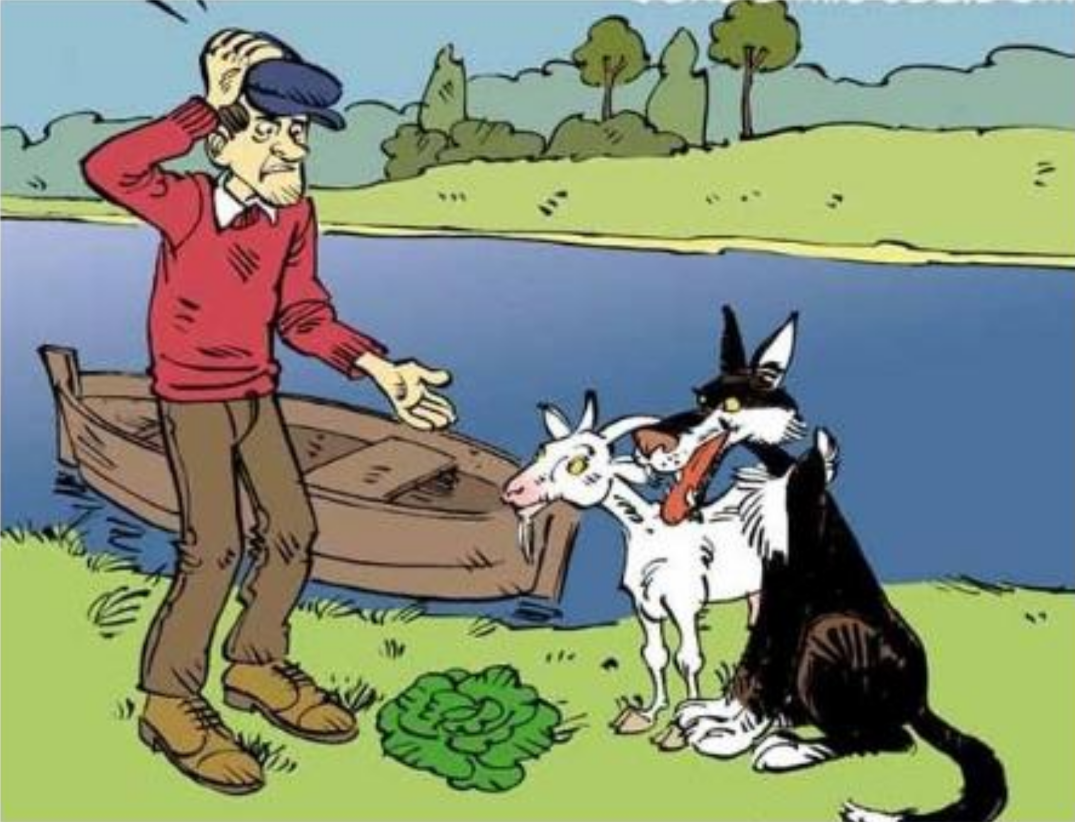
\includegraphics[width=0.38\linewidth]{Loup_chevre_chou_passeur}
	\end{center}
	\caption{Illustration du problème}
\end{figure}

On décide de représenter le passeur par la lettre P, la chèvre par la lettre C, le loup par L et le chou par X. Une situation est représentée par une chaine de caractères correspondant à l'ensemble des entités présentes sur la rive gauche.

%Un fichier \texttt{traversee\_etudiant.py} est dans votre espace de classe partagé. 
%Il définit un graphe \texttt{G} sous la forme d'un dictionnaire d'adjacence avec pour sommets les différentes situations sous forme de chaine de caractères, et, pour arêtes, les liens possibles en effectuant un trajet unique en barque d'une rive à l'autre.

\begin{figure}[h]
	\begin{center}
		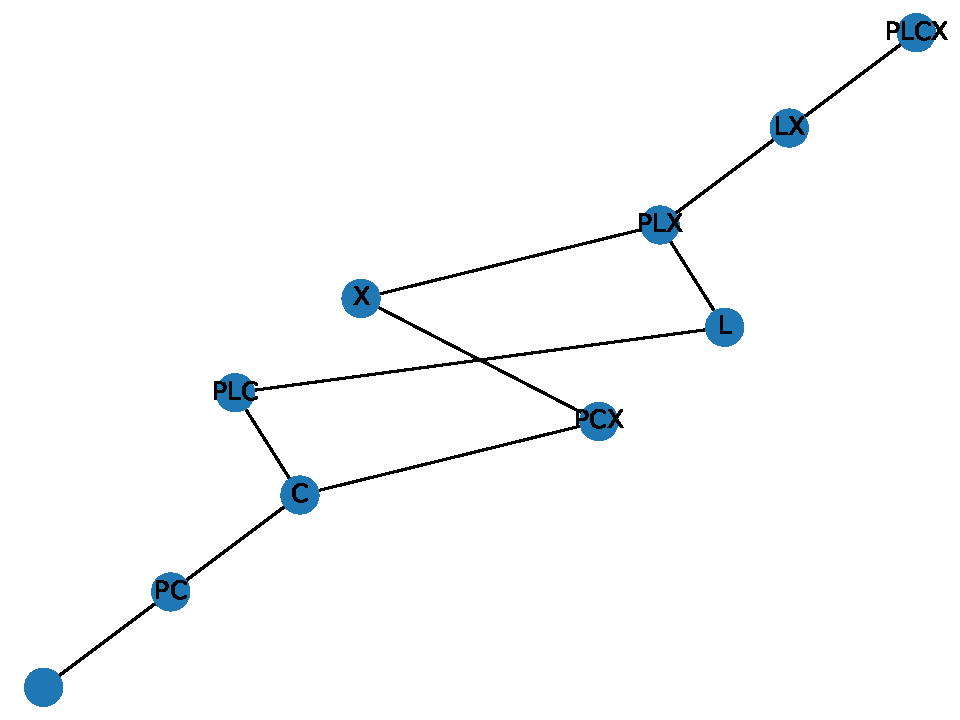
\includegraphics[width=0.38\linewidth]{Graphe_initial_passeur}
	\end{center}
	\caption{Représentation graphique du graphe \texttt{G}}
\end{figure}

\question{Définir le graphe \texttt{G} sous la forme d'un dictionnaire d'adjacence avec pour sommets les différentes situations sous forme de chaine de caractères, et, pour arêtes, les liens possibles en effectuant un trajet unique en barque d'une rive à l'autre.}

\question{\'Ecrire une fonction \texttt{existence\_chemin(G, dep, arr)} qui prend en entrée un graphe codé par un dictionnaire d'adjacence \texttt{G}, un sommet de départ \texttt{dep}, un sommet d'arrivée \texttt{arr} et renvoie un booléen~: \texttt{True} si un chemin existe entre \texttt{dep} et \texttt{arr}, \texttt{False} sinon. Pour ce faire, vous utiliserez un parcours en profondeur.}



\question{Vérifier que \texttt{existence\_chemin(G, "PLCX", "")} renvoie \texttt{True}.}



\question{\'Ecrire une fonction \texttt{trouver\_chemin(G, dep, arr)} qui renvoie une liste de sommets correspondant au chemin entre \texttt{dep} et \texttt{arr}. Vous pouvez par exemple créer un dictionnaire d'antécédent pour mémoriser le sommet d'où on vient.}





